\documentclass[11pt,american]{article}
\usepackage[letterpaper,hmargin=1.25in,vmargin=1.25in]{geometry}

\usepackage[utf8]{inputenc}
\usepackage[mathscr]{euscript}
%\usepackage[affil-it]{authblk}
\usepackage{authblk}
\usepackage{times}
\usepackage{babel}
\usepackage{url}
\usepackage{amsmath}
\usepackage{amssymb}
\usepackage{graphicx}
\usepackage{subfigure}
\usepackage{verbatim} % For comment env
\usepackage{enumerate}
\usepackage{afterpage}
\usepackage{hyperref} % For internal links
\usepackage{nag}      % Warn about old packages and commands
\usepackage{fixltx2e} % Fix misc. LaTeX stuff
\usepackage{xspace}   % Fix spacing at end of macros
\usepackage{array}
\usepackage{etoolbox}
\usepackage{multirow}
\usepackage{rotating}
\usepackage{algorithm}
\usepackage{algorithmicx}
\usepackage{algpseudocode}
\usepackage{caption}
\usepackage{float}    % 'H' table placement option
%\usepackage{compactbib} % More compact bibliography

\usepackage{tikz}
\usetikzlibrary{calc}

\setcounter{MaxMatrixCols}{16}

\newenvironment{smallpmatrix}
  {\left(\begin{smallmatrix}}
  {\end{smallmatrix}\right)}

% For now, to help organize
\setcounter{tocdepth}{5}
\newcommand{\TODO}{\textcolor{red}{\textbf{TODO}}\xspace}

\newcommand{\Ztwo}{\ensuremath{\mathbb{Z}_2}\xspace}
\newcommand{\Zn}{\ensuremath{\mathbb{Z}_n}\xspace}
\newcommand{\gftwo}{\ensuremath{\mathrm{GF}(2)}\xspace}
\newcommand{\gfsixteen}{\ensuremath{\mathrm{GF}(2^{16})}\xspace}
\newcommand{\gfwithpoly}{\ensuremath{\text{GF}(2^{16}) / \left\langle \ourpoly \right\rangle}\xspace}

\newcommand{\pval}{\textit{P-value}\xspace}
\newcommand{\pvals}{\textit{P-values}\xspace}

\newcommand{\Keccak}{\textsc{Keccak}\xspace}
\newcommand{\SpongeWrap}{\textsc{SpongeWrap}\xspace}

\newcommand{\drawxTimes}[2]{% center: x,y
  \draw[fill=gray!15,line width=2.5pt] (#1, #2) ellipse (1em and 1em) node {$x*$};
}
\newcommand{\drawXOR}[2]{% center: x,y
  \draw[fill=gray!15,line width=2.5pt] (#1, #2) ellipse (1em and 1em);
  \draw[line width=2.5pt] (#1-.4, #2) -- (#1+.4, #2);
  \draw[line width=2.5pt] (#1, #2-.4) -- (#1, #2+.4);
}
\newcommand{\drawAdder}[2]{% top left: x,y
  \draw[fill=gray!15,line width=2.5pt] (#1, #2) rectangle (#1+1, #2-1);
  \draw[line width=2.5pt] (#1, #2-.5) -- (#1+1, #2-.5);
  \draw[line width=2.5pt] (#1+.5, #2-1) -- (#1+.5, #2);
}
\newcommand{\drawRot}[2]{% center: x,y
  \draw[fill=gray!15,line width=2.5pt] (#1, #2) ellipse (2em and 1em) node {$\mathbf{ROT}$};
}
\newcommand{\drawMixerInputs}{
  \draw[fill=gray!30] (0,16) rectangle (2,15) node[midway] {$A$};
  \draw[fill=gray!30] (4,16) rectangle (6,15) node[midway] {$B$};
}
\newcommand{\drawMixerOutputs}[1]{%y offset from top
  \draw[fill=gray!30] (0,16-#1) rectangle (2,15-#1) node[midway] {$A'$};
  \draw[fill=gray!30] (4,16-#1) rectangle (6,15-#1) node[midway] {$B'$};
}

% Aliases for readability
\let\from=\colon
\let\to=\rightarrow

% TODO better title
%\title{A Customizable Sponge-Based Authenticated Encryption Algorithm with $16$-bit S-boxes}
\title{Customizable Sponge-Based Authenticated Encryption Using $16$-bit S-boxes}
%\author{Matthew Kelly
        %\and Alan Kaminsky
        %\and Marcin {\L}ukowiak
        %\and Michael Kurdziel
        %\and Stanis{\l}aw Radziszowski}
\author[1]{Matthew Kelly}
\author[2]{Alan Kaminsky}
\author[1]{Marcin {\L}ukowiak}
\author[3]{\authorcr Michael Kurdziel}
\author[2]{Stanis{\l}aw Radziszowski}
%\affil[1]{\footnotesize Department of Computer Engineering, \authorcr Rochester Institute of Technology}
\affil[1]{\footnotesize Department of Computer Engineering, Rochester Institute of Technology}
%\affil[2]{Department of Computer Science,  \authorcr Rochester Institute of Technology}
\affil[2]{Department of Computer Science, Rochester Institute of Technology}
\affil[3]{Harris Corporation, Rochester, NY}

\date{September 2014}

\begin{document}

\maketitle
%\footnote{\TODO Harris acknowledgement?}

\begin{abstract}
Authenticated encryption (AE) is a symmetric key cryptographic scheme that aims to provide both confidentiality and data integrity. 
There are many AE algorithms in existence today.
However, they are often far from ideal in terms of efficiency and ease of use.
For this reason, there is ongoing effort to develop new AE algorithms that are secure, efficient, and easy to use.

The sponge construction is a relatively new cryptographic primitive that has gained popularity since the SHA-3 hashing competition was won by the sponge-based \Keccak algorithm.
The duplex construction, which is closely related to the sponge, provides promising potential for secure and efficient authenticated encryption.

In this paper we introduce a novel authenticated encryption algorithm based on the duplex construction that is targeted for hardware implementation.
We also provide explicit customization guidelines for users who desire unique authenticated encryption solutions within our security margin.
Futhermore, our substitution step uses $16 \times 16$ AES-like S-boxes.
We believe this to be the first algorithm in the literature to use such large bijective S-boxes.
\end{abstract}

%------------------------------
% SECTION: Introduction
%------------------------------
\section{Introduction}
The overarching goal of symmetric key cryptography is to enable people to communicate privately over an insecure channel in the presence of adversaries.
Two fundamental requirements for achieving this goal are encryption and authentication.
Encryption provides \emph{confidentiality} while authentication provides data \emph{integrity} and assurance of message origin.

Many authenticated encryption algorithms are in existence today, but they are often unsatisfactory in terms of performance, security, or ease of use.
Some algorithms require two passes per block of plaintext to encrypt and authenticate.
This is generally undesirable because it often means a much slower algorithm.
Other algorithms have been shown to be insecure or difficult to use properly.
Many algorithms, such as the ones based on generic composition, require two keys.
This should be avoided when possible because key management is a difficult problem.

Furthermore, a new authenticated encryption algorithm is needed that meets the stringent requirements of government and military applications.
Such algorithms are not typically in the public domain.
The goal of this is partially to reduce or eliminate academic interest in cryptanalyzing the algorithm and publishing results.
This stance is highly controversial.
Still, the security of such algorithms depends entirely on the secrecy of the key and not on the secrecy of the algorithm.
The assumption is still made that the enemy knows the details of the algorithm being used at any time \cite{Kurdziel2002_BaselineRequirements}.

For this reason, there is a need for a customizable authenticated encryption algorithm.
This algorithm should remain secure as long as customizations are made within certain guidelines.
The result is an algorithm which can be made unique on a per-user or per-application basis without the effort of cryptanalyzing every specific instantiation.
We present such an algorithm here.


%------------------------------
% SECTION: Sponge and Duplex Constructions 
%------------------------------
\section{Sponge Construction}
\label{sec:SpongeAndDuplex}
The sponge construction is a relatively new cryptographic primitive that has gained popularity since \Keccak won the Secure Hash Algorithm (SHA-3) competition in 2013 \cite{Bertoni2011_KeccakReference}\cite{NIST2012_SHA3_Winner}.
Essentially, it provides a way to generalize hash functions (which normally have outputs of fixed length) to functions with arbitrary length output.
This generalization allows cryptographic sponges to be used for applications other than hashing.

Sponges are based on the iteration of an underlying function $f$.
This function can either be a general \emph{transformation} or a \emph{permutation}.
The security proofs are different for transformations and permutations, and there are advantages and disadvantages for each choice of a function type \cite{Bertoni2011_SpongeFunctions}.

%\subsection{Sponge Parameters}
The output $Z$ of the parameterized sponge construction is given as
\begin{equation*}
\label{eq:SpongeOutput}
Z = \mathbf{sponge}[f,\mathbf{pad},r](M,\ell),
\end{equation*}
where $\mathbf{pad}$ is a padding function for the input, $r$ is the \emph{rate} of absorption, $M$ is the message (or other input) data, and $\ell$ is the desired output length.
The sponge construction is stateless; there is no information stored between calls to it.
It is split into two distinct phases: the \emph{absorbing} phase and the \emph{squeezing} phase.
Inputs (e.g.\ message and/or key material) are absorbed in the first phase and the output (e.g.\ a MAC or keystream) is squeezed out in the second phase.

The state of the sponge construction is split into two contiguous portions: the \emph{outer state}, which is accessible externally, and the \emph{inner state}, which is hidden.
The size of the outer state is given by the \emph{rate} $r$ and the size of the inner state is specified by the \emph{capacity} $c$.
The size of the entire state is $b = r + c$.
The speed of the construction depends on the rate, while the security depends on the capacity.

The padding function $\mathbf{pad}$ is first applied to $M$ to make it a multiple of $r$.
$M$ is then absorbed $r$ bits at a time.
More concretely, absorption is the process of XORing $r$-bit blocks into the state while interleaving with applications of the underlying sponge function $f$.
If the rate is increased then more bits are absorbed at a time and thus the construction runs faster.
However, increasing the rate means that the capacity must decrease and so there is a clear trade-off between speed and security.
Squeezing consists of concatenating $r$ bits at a time to an output bitstring $Z$ that is truncated to $\ell$ bits.
The sponge function $f$ must be called once for each $r$ bits of output after the first full block.

%------------------------------
% SECTION:Duplex Construction
%------------------------------
\section{Duplex Construction}
The duplex construction is highly related to the sponge construction.
The main differences are that the duplex construction maintains state between calls and that there no longer exists a clear separation between the absorbing and squeezing phases.
Absorbing and squeezing happen essentially at the same time, hence ``duplexing'' \cite{Bertoni2012_Duplexing}.
The duplex mode has several applications \cite{Bertoni2010_DuplexingSlides}, with authenticated encryption being the one of obvious interest to us.

%\subsection{Duplex Parameters}
Parameters for the duplex construction are mostly the same as for the sponge construction.
However, since the duplex construction maintains state, we build a \emph{duplex object} $D$ and make calls to it.
The function which processes inputs and produces outputs is called $\mathbf{duplexing}$:
\begin{equation*}
Z_i = D.\mathbf{duplexing}(\sigma_i,\ell_i)
\end{equation*}

\begin{figure}[ht]
\centering
\includegraphics[width=0.8\textwidth]{img/Duplex.pdf}
\caption{The duplex construction $\mathbf{duplex}[f,\mathbf{pad},r]$ \cite{Bertoni2011_SpongeFunctions}}
\label{fig:Duplex}
\end{figure}
Figure~\ref{fig:Duplex} shows the duplex construction.
The $i$-th input is denoted $\sigma_i$ and the $i$-th output is denoted $Z_i$, which is truncated to $\ell_i$ bits.
Inputs are absorbed and processed at the same time that outputs are squeezed.
For a duplex object it is possible to have an empty input or to not request an output.
A \emph{blank call} is a call to $\mathbf{duplexing}$ for which no input is provided ($|\sigma_i| = 0$).
A \emph{mute call} is a call for which no output is requested ($\ell_i = 0$).

\subsection{Duplex for Authenticated Encryption}
Authenticated encryption is easily achieved using the duplex construction.
Figure~\ref{fig:DuplexAE_Expanded} shows such a use case.
First, we construct a duplex object $D$.
Then we absorb the key $K$ (or optionally $K||IV$) using one or more mute calls to $D.\mathbf{duplexing}$.
More that one mute call may be required if the length of the key exceeds the rate $r$.
We denote a header input to $D$ as $A$; these arbitrary length inputs are authenticated but not encrypted.
We denote a body input to $D$ as $B$; these arbitrary length inputs are both encrypted and authenticated.
$A$ inputs are absorbed using one or more mute calls to $D.\mathbf{duplexing}$.
$B$ inputs are absorbed in a similar fashion and then the keystream $Z$ is XORed with $B$ to produce the ciphertext $C$.
The tag $T$ is produced using a blank call to $D.\mathbf{duplexing}$ after all header and body inputs have been processed.

\begin{figure}[ht]
\centering
\includegraphics[width=0.8\textwidth]{img/DuplexAE_Expanded-BW.png}
\caption{The duplex construction as used for authenticated encryption \cite{Bertoni2010_DuplexingSlides}}
\label{fig:DuplexAE_Expanded}
\end{figure}

\begin{comment}
\begin{enumerate}
\item Easy to use
\item Single key required
\item Single-pass for encryption and authentication
\item Support for intermediate tags
\item Support for Additional Authenticated Data (AAD, or headers)
\item Secure against generic attacks
\item Ability to trade off speed and security by adjusting $r$
\end{enumerate}
\end{comment}

We note that the duplex construction may require \emph{domain separation}, a generic mechanism for eliminating output ambiguity.
For example, the simplest domain separation method consists of appending a \emph{frame bit} to the last block of every different input data type (e.g.\ key or message data).
This frame bit has the property that no two consecutive data types have the same frame bit value, meaning that one can easily identify where one data type ends and the next begins \cite{Bertoni2012_Duplexing}.

\subsection{Generic Security}
\label{sec:DuplexSecurity}
Any calls made to the duplex construction can be reduced to calls to the keyed sponge construction.
As a result, the security of the duplex construction depends only on its corresponding sponge construction.

The security of the sponge construction is based on the assumption that the underlying sponge function $f$ is secure.
That is, if $f$ is computationally indistinguishable from random then so should be the sponge construction it is instantiated within.
Consequently, cryptographers designing a system based on the sponge construction need only be concerned with designing and cryptanalyzing a secure underlying function.
The sponge construction, when used properly, is said to be secure against \emph{generic attacks} -- attacks which do not exploit any specific properties of the underlying sponge function.
We call this the \emph{generic security} of the construction \cite{Bertoni2011_SpongeFunctions}.

The generic security of keyed constructions is higher than unkeyed.
For our purposes we are interested only in the security of the keyed sponge construction where a permutation is used for $f$. 
Jovanovic et.~al\ \cite{Jovanovic2014_Beyond} proved in 2014 that the generic security level of keyed sponge constructions is lower bounded by 
\begin{equation*}
\mathrm{min}(2^{(r+c)/2}, 2^c, 2^{|K|}).
\end{equation*} 


%%%%%%%%%%%%%%%%%%%%%%%%%%%%%%%%%%%%
% Section: Our Algorithm 
%%%%%%%%%%%%%%%%%%%%%%%%%%%%%%%%%%%%
\section{Our Algorithm}
\begin{frame}
\frametitle{Algorithm Overview}
\begin{itemize}
  \item Based on the simplified duplex construction with parameters:
  \begin{itemize}
    \item Width: $b = 512$
    \item Rate: $r = 128$ 
    \item Capacity: $c = 384$ 
  \end{itemize}
  \item Most design effort into pseudorandom permutation $f$
\end{itemize}
\end{frame}

\begin{frame}
\frametitle{Permutation Overview}
\begin{itemize}
  \item Permutation consists of several \emph{rounds}
  \begin{itemize}
    \item $R = 10$ for $128$-bit key
    \item $R = 16$ for $256$-bit key
  \end{itemize}
  \item Each round consists of 4 steps
  \begin{itemize}
    \item Substitution
    \item Bitwise Permutation
    \item Mixer
    \item Add Round Constant
  \end{itemize}
  \item Each step has a fairly specific purpose
\end{itemize}
\end{frame}

% TODO might be impossible to make this look good
\begin{comment}
\begin{frame}
\frametitle{Single Round Illustrated}
\begin{figure}[p]
\centering
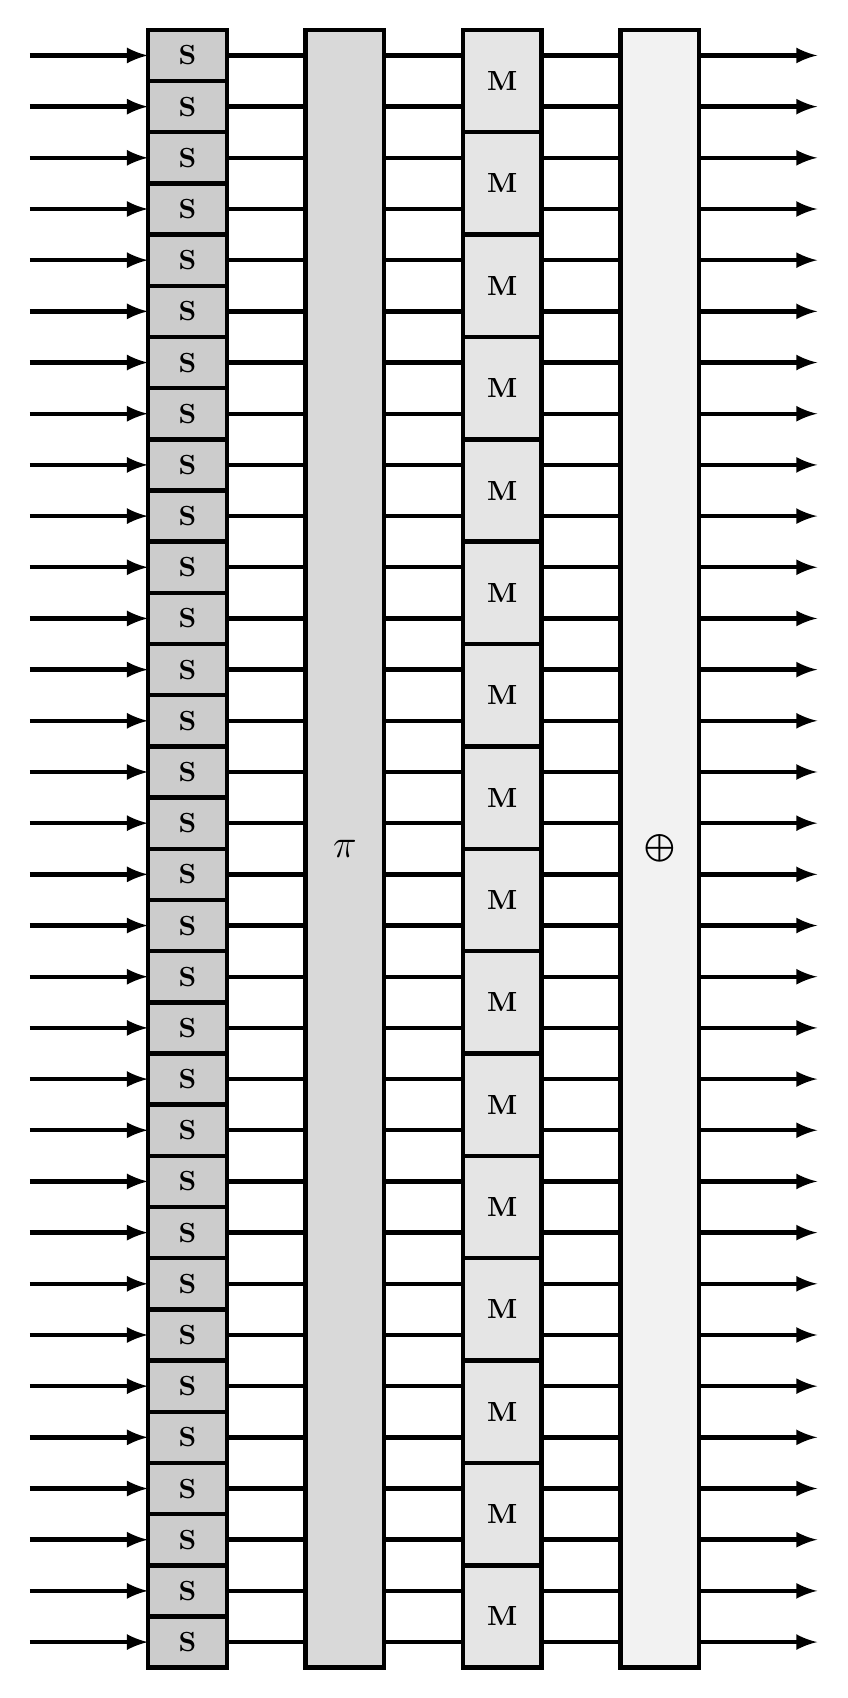
\begin{tikzpicture}[xscale=1,yscale=0.65,>=latex,ultra thick]
% Reference grid (temporary)
%\draw[help lines] (0,0) grid (16,32);

% TODO label bits / words

% Entry arrows
\foreach \i in {32,...,1} {
  \draw[->] (-1.5,\i-0.5) -- (0,\i-0.5);
}

% Wires
\foreach \j in {1,3,5} {
  \foreach \i in {32,...,1} {
    \draw (\j,\i-0.5) -- (\j+1,\i-0.5);
  }
}

% S-boxes
\foreach \i in {32,...,1} {
  \draw[fill=gray!40] (0,\i) rectangle (1,\i-1) node[midway] {$\mathbf{S}$} ;
}

% P-boxes
\draw[fill=gray!30] (2,0) rectangle (3,32) node[midway] {\Large$\mathbf{\pi}$};

% Mixers
\foreach \i in {32,30,...,2} {
  \draw[fill=gray!20] (4,\i) rectangle (5,\i-2) node[midway] {$\mathbf{M}$};
}

% Round key box
\draw[fill=gray!10] (6,0) rectangle (7,32) node[midway] {$\bigoplus$};

% Exit arrows
\foreach \i in {32,...,1} {
  \draw[->] (7,\i-0.5) -- (8.5,\i-0.5);
}

\end{tikzpicture}


\caption{A single round of the sponge permutation $f$. Each line represents a $16$-bit word.}
\end{figure}
\end{frame}
\end{comment}

\begin{frame}
\frametitle{Single Round Illustrated}
\vfill
\begin{center}
\Large
See thesis document...sorry!
\end{center}
\vfill
\end{frame}

\begin{frame}
\frametitle{Substitution Step}
\begin{itemize}
  \item \emph{S-box}: random-looking map from $n$-bit inputs to $m$-bit outputs
  \item Main source of \emph{confusion} 
  \item We use 32 identical $16 \times 16$ S-boxes
  \item Could be randomly generated mappings with nice properties
  \begin{itemize}
    \item Not suitable for hardware
  \end{itemize}
  \item Instead based on invertible operations in a GF (similar to AES)
\end{itemize}
\end{frame}

\begin{frame}
\frametitle{S-box}
\begin{itemize}
  \item Taken from Chris Wood's MS thesis (CS Dept., 2013) \cite{Wood2013_SboxThesis}
  \item Multiplicative inversion in \gfsixteen with irreducible polynomial
  \begin{equation*}
    p(x) = x^{16} + x^5 + x^3 + x + 1
  \end{equation*} 
  \item Followed by affine transformation
  \begin{itemize}
    \item Increase algebraic complexity
  \end{itemize}
  \item Only 1238 XOR gates and 144 AND gates in hardware
\end{itemize}
\end{frame}

\begin{frame}
\frametitle{S-box Equation}
\begin{equation*}
\footnotesize
%\renewcommand{\arraystretch}{0.7} % Make it square
\begin{pmatrix}
0 & 0 & 1 & 0 & 0 & 0 & 0 & 1 & 0 & 0 & 1 & 1 & 1 & 1 & 1 & 0 \\
1 & 1 & 0 & 0 & 0 & 0 & 0 & 1 & 0 & 1 & 1 & 0 & 1 & 0 & 1 & 0 \\
1 & 1 & 0 & 0 & 1 & 0 & 1 & 1 & 0 & 1 & 0 & 1 & 0 & 0 & 1 & 1 \\
1 & 1 & 1 & 0 & 0 & 0 & 1 & 0 & 0 & 1 & 1 & 0 & 0 & 0 & 0 & 0 \\

1 & 1 & 0 & 0 & 0 & 1 & 1 & 0 & 0 & 1 & 1 & 1 & 1 & 0 & 1 & 1 \\
0 & 1 & 0 & 0 & 0 & 0 & 1 & 1 & 0 & 1 & 1 & 1 & 1 & 1 & 0 & 1 \\
0 & 0 & 1 & 0 & 1 & 0 & 1 & 0 & 1 & 1 & 0 & 0 & 1 & 1 & 0 & 0 \\
1 & 0 & 1 & 1 & 1 & 0 & 1 & 1 & 0 & 0 & 0 & 1 & 0 & 1 & 1 & 1 \\

0 & 1 & 0 & 0 & 0 & 0 & 0 & 0 & 1 & 0 & 0 & 1 & 1 & 1 & 0 & 1 \\
1 & 0 & 1 & 1 & 0 & 0 & 0 & 1 & 0 & 0 & 1 & 0 & 1 & 0 & 0 & 0 \\
1 & 0 & 1 & 0 & 0 & 1 & 1 & 1 & 0 & 0 & 1 & 1 & 0 & 1 & 0 & 0 \\
1 & 0 & 1 & 1 & 1 & 0 & 1 & 1 & 1 & 1 & 0 & 1 & 1 & 0 & 0 & 1 \\

1 & 0 & 1 & 0 & 0 & 1 & 0 & 1 & 1 & 0 & 0 & 1 & 0 & 0 & 0 & 1 \\
0 & 1 & 0 & 0 & 0 & 1 & 1 & 1 & 1 & 0 & 0 & 0 & 0 & 0 & 0 & 1 \\
1 & 0 & 0 & 0 & 1 & 1 & 0 & 1 & 0 & 1 & 1 & 1 & 1 & 0 & 0 & 0 \\
1 & 1 & 0 & 1 & 0 & 1 & 1 & 0 & 1 & 0 & 0 & 1 & 1 & 0 & 0 & 0 \\
\end{pmatrix}
\begin{pmatrix}
x_{15} \\
x_{14} \\
x_{13} \\
x_{12} \\
x_{11} \\
x_{10} \\
x_{9} \\
x_{8} \\
x_{7} \\
x_{6} \\
x_{5} \\
x_{4} \\
x_{3} \\
x_{2} \\
x_{1} \\
x_{0} \\
\end{pmatrix}
^{-1}
\oplus
\begin{pmatrix}
0 \\
1 \\
0 \\
0 \\
0 \\
1 \\
0 \\
1 \\
1 \\
0 \\
1 \\
1 \\
0 \\
1 \\
1 \\
1 \\
\end{pmatrix}
\end{equation*}
\end{frame}

\begin{frame}
\frametitle{Inverse S-box Equation}
\begin{equation*}
\footnotesize
%\renewcommand{\arraystretch}{0.7} % Make it square
\left[
\begin{pmatrix}
0 & 1 & 0 & 1 & 0 & 1 & 1 & 1 & 0 & 0 & 1 & 0 & 0 & 0 & 0 & 1 \\
1 & 1 & 0 & 1 & 0 & 0 & 1 & 0 & 1 & 0 & 1 & 1 & 1 & 1 & 0 & 1 \\
1 & 0 & 1 & 1 & 1 & 1 & 0 & 1 & 0 & 1 & 1 & 0 & 0 & 0 & 0 & 0 \\
0 & 0 & 1 & 0 & 1 & 1 & 1 & 0 & 1 & 0 & 1 & 1 & 1 & 0 & 1 & 0 \\

1 & 1 & 1 & 1 & 1 & 0 & 0 & 0 & 1 & 0 & 0 & 0 & 0 & 1 & 0 & 0 \\
0 & 0 & 0 & 1 & 0 & 1 & 0 & 0 & 0 & 0 & 1 & 1 & 1 & 1 & 1 & 1 \\
1 & 0 & 1 & 0 & 0 & 0 & 0 & 0 & 0 & 1 & 1 & 0 & 1 & 0 & 1 & 1 \\
0 & 0 & 1 & 0 & 1 & 1 & 1 & 0 & 0 & 1 & 0 & 1 & 1 & 1 & 1 & 0 \\

0 & 0 & 0 & 0 & 0 & 0 & 1 & 0 & 0 & 0 & 1 & 0 & 0 & 0 & 1 & 0 \\
1 & 1 & 1 & 0 & 0 & 1 & 1 & 1 & 1 & 0 & 1 & 1 & 1 & 0 & 0 & 0 \\
0 & 1 & 1 & 0 & 1 & 1 & 1 & 1 & 0 & 0 & 1 & 0 & 1 & 1 & 1 & 1 \\
1 & 0 & 0 & 1 & 1 & 0 & 0 & 0 & 1 & 0 & 0 & 1 & 1 & 0 & 1 & 1 \\

1 & 0 & 0 & 0 & 0 & 1 & 0 & 1 & 1 & 1 & 0 & 0 & 1 & 0 & 1 & 0 \\
1 & 0 & 0 & 0 & 0 & 1 & 1 & 1 & 1 & 1 & 0 & 1 & 1 & 1 & 1 & 1 \\
1 & 1 & 1 & 0 & 0 & 1 & 1 & 0 & 1 & 0 & 0 & 1 & 1 & 1 & 1 & 1 \\
0 & 1 & 0 & 0 & 1 & 0 & 1 & 0 & 1 & 0 & 0 & 1 & 0 & 0 & 0 & 1 \\
\end{pmatrix}
\begin{pmatrix}
x_{15} \\
x_{14} \oplus 1 \\
x_{13} \\
x_{12} \\
x_{11} \\
x_{10} \oplus 1 \\
x_{9} \\
x_{8} \oplus 1 \\
x_{7} \oplus 1 \\
x_{6} \\
x_{5} \oplus 1 \\
x_{4} \oplus 1 \\
x_{3} \\
x_{2} \oplus 1 \\
x_{1} \oplus 1 \\
x_{0} \oplus 1 \\
\end{pmatrix}
\right]^{-1}
\end{equation*}
\end{frame}

\begin{frame}
\frametitle{Bitwise Permutation}
\begin{itemize}
  \item Provides \emph{long-range diffusion}
  \item Aims to increase min number of active S-boxes
  \item Could be random mapping with nice properties
  \item We define it using an affine function with nice properties
  \item Allows for compact representation
  \begin{equation*}
  \pi(x) = 31x + 15 \pmod{512}
  \end{equation*}
  where $x \in \mathbb{Z}_{512}$ is the bit index
\end{itemize}
\end{frame}

\begin{frame}
\frametitle{Bitwise Permutation Properties}
\begin{enumerate}
  \item Sends all $16$ outputs of each S-box to 16 different mixers
  \item Has no fixed points: $\pi(x) \ne x$ for any $x$
  \item High order; does not repeat within $R$ rounds
  \item No lower order bits
\end{enumerate}
We found $384$ permutations defined by affine functions that satisfy these properties.
\end{frame}

\begin{frame}
\frametitle{PRESENT Attack}
\begin{figure}[ht]
\centering
\includegraphics[height=0.62\textheight]{img/PRESENT_Trail.png}
\caption{Minimization of PRESENT active S-boxes}
\end{figure}
\end{frame}

\begin{frame}
\frametitle{Mixer}
\begin{itemize}
  \item Increase \emph{branch number} of round to 3
  \begin{itemize}
    \item Verified via SAT solver analysis 
    \item Tools courtesy of Alan Kaminsky
  \end{itemize}
  \item Provide local diffusion
  \item Defined by invertible matrix multiplication in \gfsixteen
  \item Irreducible polynomial:
  \begin{equation*}
  p(x) = x^{16} + x^5 + x^3 + x^2 + 1
  \end{equation*}
\end{itemize}
\end{frame}

\begin{frame}
\frametitle{Mixer Equations}
\begin{itemize}
  \item Input two words $A$ and $B$
  \item Forward:
  \begin{equation*}
  \begin{pmatrix}
  A' \\ B'
  \end{pmatrix}
  =
  \begin{pmatrix}
  1 & x \\ x & x + 1
  \end{pmatrix}
  \begin{pmatrix}
  A \\ B
  \end{pmatrix}
  \end{equation*}
  
  \item Inverse: 

\begin{equation*}
\begin{pmatrix}
A \\ B
\end{pmatrix}
=
\begin{pmatrix}
a & b \\ b & c
\end{pmatrix}
\begin{pmatrix}
A' \\ B'
\end{pmatrix}
\end{equation*}
where
\begin{align*}
a &= x^{15} + x^{14} + x^{12} + x^{11} + x^9 + x^8 + x^6 + x^5 + x^4 + x + 1 \\
b &= x^{14} + x^{13} + x^{11} + x^{10} + x^8 + x^7 + x^5 + x^4 + x^3 + 1 \\
c &= x^{15} + x^{13} + x^{12} + x^{10} + x^9 + x^7 + x^6 + x^3 + x.
\end{align*}
\end{itemize}
\end{frame}

\begin{frame}
\frametitle{Mixer in Hardware}
\begin{figure}[ht]
\centering
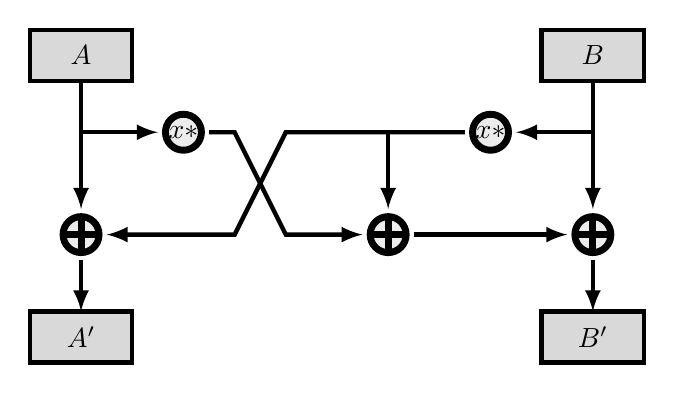
\begin{tikzpicture}[xscale=0.65,yscale=0.65,>=latex,ultra thick]
% Reference grid (temporary)
%\draw[help lines] (0,0) grid (16,16);

% Inputs
\draw[fill=gray!30] (0,15) rectangle (2,14) node[midway] {$A$};
\draw[fill=gray!30] (10,15) rectangle (12,14) node[midway] {$B$};

\draw[->] (1,14) to (1, 11.5);
\draw[->] (1,13) to (2.5, 13);

\draw[->] (11,14) to (11, 11.5);
\draw[->] (11,13) to (9.5, 13); 

\drawxTimes{3}{13}
\drawxTimes{9}{13}

\drawXOR{1}{11}
\drawXOR{11}{11}
\drawXOR{7}{11}

\draw[->] (3.5,13) to (4,13) to (5,11) to (6.5,11);
\draw[->] (8.5,13) to (5,13) to (4,11) to (1.5,11); 
\draw[->] (7,13) to (7,11.5);
\draw[->] (7.5,11) to (10.5,11);

\draw[->] (1,10.5) to (1,9.5);
\draw[->] (11,10.5) to (11,9.5);

% Outputs
\draw[fill=gray!30] (0,9.5) rectangle (2,8.5) node[midway] {$A'$};
\draw[fill=gray!30] (10,9.5) rectangle (12,8.5) node[midway] {$B'$};

\end{tikzpicture}

\caption{Hardware implementation of forward mixer function.}
\end{figure}
\end{frame}

\begin{frame}
\frametitle{$x*$ in Hardware}
\begin{figure}[ht]
\centering
\includegraphics[width=\textwidth]{img/xTimes.pdf}
\caption{Hardware implementation of the $x*$ function. The leftmost bit is the MSB.}
\end{figure}
\end{frame}

\begin{frame}
\frametitle{Add Round Constant}
\begin{itemize}
  \item Very simple; its own inverse
  \item Bitwise XOR $512$-bit round constant into state
  \item Reduces symmetry in state
  \item Prevents against \emph{slide attacks}
  \item RCs generated as follows:
  \begin{equation*}
  RC_i = \mathbf{SHA3\textbf{-}512}(\mathbf{ASCII}(i))
  \end{equation*}
\end{itemize}
\end{frame}

\begin{frame}
\frametitle{Customization}
\begin{itemize}
  \item Different S-box from Wood's thesis
  \begin{itemize}
    \item Recalculate maximum linear bias and differential probabilities
  \end{itemize}
  \item Different bitwise permutation out of the $384$ we found
  \item Different matrix for mixer
  \begin{itemize}
    \item Verify branch number is 3 using SAT tools 
  \end{itemize} 
  \item Different round constants
\end{itemize}
\end{frame}


%------------------------------
% SECTION: Preliminary Cryptanalysis
%------------------------------
\section{Comments on Cryptanalysis}
\label{sec:Cryptanalysis}
The duplex construction has been shown to be secure against generic attacks by the \Keccak team \cite{Bertoni2011_SpongeFunctions}.
Therefore it is sufficient for us to assess only the security of the underlying sponge permutation $f$.

We provide an overview of our preliminary cryptanalysis here.
Emphasis is placed on the most general and prevalent forms of attacks.
Resistance against these techniques should result in resistance against many other less general techniques.
Our aim is to provide intuitive explanations of prevalent methods and simply explain why our permutation should be resistant.
Further cryptanalysis, as with all cryptosystems, is always welcome as future work.

%------------------------------
% Differential Cryptanalysis
%------------------------------
\subsection{Differential Cryptanalysis}
Differential cryptanalysis was publicly introduced by Biham and Shamir in 1991 in their landmark paper on the subject \cite{Biham1991_Differential}.
Since then, it has been applied with varying degrees of success to a great number of cryptosystems.
As such, it is a fundamental requirement of symmetric key cryptosystem design to prove resistance to differential cryptanalysis.

To determine the resistance of our algorithm to differential cryptanalysis, we first have to determine the maximum differential probability of our S-box.
We determined this value to be $p_{D,max} = 2^{-14}$ using an S-box evaluation program called \texttt{Eval16BitSbox} \cite{Kaminsky2014_BlockCipherAnalysis} written with Kaminsky's Parallel Java 2 library \cite{Kaminsky2014_PJ2}.

Next, it is necessary to determine the differential branch number of a round.
For this, we only need to analyze the mixer. 
We purposefully designed a mixer with differential branch number equal to three, meaning that minimally three S-boxes will be differentially active between two rounds.
This is in fact the maximum achievable branch number for a transformation defined by multiplication by a $2 \times 2$ matrix.
To verify this, we used a SAT solver called CryptoMiniSat \cite{Soos2014_CryptoMiniSat}.
This SAT solver takes as input a Boolean equation in conjunctive normal form (CNF) and determines if it is satisfiable.
Our CNFs were generated using Kaminsky's \texttt{SatProblem} Java class \cite{Kaminsky2014_BlockCipherAnalysis}.

The CNFs generated are unsatisfiable if and only if the mixer has differential branch number equal to three since it answers the following question (refer to Figure~\ref{fig:MixerMatrix}): \emph{is it possible to have a difference in only one input ($A$ or $B$) and only one output ($A'$ or $B'$)?}
Through SAT solver analysis we determined that this is not possible for our mixer; that is, if there is a non-zero difference in either $A$ or $B$, there must be a non-zero difference in both $A'$ and $B'$.
In the event that there is a difference in both inputs, there may be a difference in only one output.
This still leads to a differential branch number of three since two S-boxes must have been active in the previous round to lead to those two input differences.
The probability of a difference in either output is $p_{D,out} = 2^{-15}$.

With all of this information, it is possible to calculate the number of rounds needed for resistance to differential attacks.
The worst-case probability of successfully propagating a difference over two rounds is given by
\begin{equation*}
(p_{D,max})^{\mathcal{B}_D} \cdot p_{D,out},
\end{equation*}
where $\mathcal{B}_D = 3$ is the differential branch number.
Next, we found that the complexity of a differential attack exceeds the complexity of a brute force attack at six rounds for a $128$-bit key.
To increase our security margin significantly, we require $10$ rounds for a $128$-bit key. 
For a $256$-bit key, $16$ rounds are required to achieve a similar security margin.

%------------------------------
% Linear Cryptanalysis
%------------------------------
\subsection{Linear Cryptanalysis}
Linear Cryptanalysis was first introduced by Matsui in 1993 in his seminal paper on the subject \cite{Matsui1993_Linear}.
As with differential cryptanalysis, it is a fundamental requirement of symmetric key cryptosystem design to prove resistance against linear attacks.

Recall that we have verified via SAT solver analysis that the differential branch number of our mixer is three.
In \cite{Daemen2002_DesignOfRijndael}, Daemen and Rijmen prove the following result: the linear branch number of a linear transformation specified by multiplication by a matrix $M$ is equal to the differential branch number of the linear transformation specified by the transpose of that matrix.
Therefore, a sufficient condition for the differential and linear branch numbers to be equal is that the matrix is symmetric.
Our matrix is symmetric and therefore we know that $\mathcal{B}_D = \mathcal{B}_L$.

The final step to prove the resistance of our algorithm against linear cryptanalysis involves determining the linear bias of two complete rounds of our permutation.
To combine linear biases, we use Matsui's Piling-Up Lemma from \cite{Matsui1993_Linear}:
\begin{equation*}
\epsilon = 2^{n-1} \prod\limits_{i = 1}^n \epsilon_i,
\end{equation*}
where $n = 3$ is the number of linearly active S-boxes across two rounds and $\epsilon_i = \epsilon_{L,max} = 2^{-8}$ is the worst case linear bias of those S-boxes.
Also from Matsui's paper, we know that the number of plaintext/ciphertext pairs (again referred to loosely as the \emph{complexity}) needed to exploit the overall bias $\epsilon$ is approximately $\epsilon^{-2}$.
Using this information, we determined that the complexity of a linear attack exceeds the complexity of a brute force search of a $128$-bit keyspace at six rounds.

\subsection{Algebraic Attacks}
Differential and linear cryptanalysis take a probabilistic approach to estimating the behavior of a system.
In contrast, algebraic attacks take a deterministic approach in that they aim to find mathematical models of a system that hold with probability $1$.
For example, in 2001 Ferguson et~al.\ \cite{Ferguson2001_AlgebraicRijndael} introduced an elegant and complete algebraic representation of AES.
The ability to create such a simple mathematical representation of the cipher initially raised alarm throughout the cryptographic community.
However, the security of AES seems to be uncompromised since we believe it is far too difficult to solve such an algebraic system - the algebraic complexity of the AES S-box is too high.

Until there are any reasons to believe otherwise, it seems that these algebraic attacks would be highly ineffective against our permutation $f$.
Even if there were a practical algebraic attack demonstrated on AES, which all literature indicates as highly implausible right now, the much larger size of our S-box and therefore the much higher algebraic complexity (see \cite{Wood2013_SboxThesis}) leads us to conjecture that our permutation would still be resistant.


%-----------------------------------
% SECTION: Conclusions 
%-----------------------------------
\section{Conclusions}
In this paper we presented a customizable authenticated encryption algorithm based on the duplex construction that is targeted for hardware implementation.
We believe this algorithm to be highly secure against known attacks.
In particular, we provided proof of resistance against linear and differential attacks as well as solid reasoning for resistance against algebraic attacks.

\subsection{Future Work}
There are two primary areas for further work relating to the algorithm presented here.
As with all cryptosystems, further cryptanalysis is always appreciated.
In particular, it would be interesting to determine the best possible linear and differential trails across several rounds.

The other area of work is the hardware implementation of the algorithm described here.
In particular, quantitative results relating to the resource usage for an FPGA implementation are of great interest.
We are confident that our permutation is designed in such a way that a relatively small amount of resources will be required.

\begin{comment}
In addition to further cryptanalysis, more analysis should be performed on similar $2 \times 2$ matrices so that a list of drop-in replacements within our security margin is readily available.
It is desirable to perform statistical analysis on the remaining $16$-bit S-boxes provided by Wood.
Knowing their maximum linear biases and differential probabilities would likely allow them to act as drop-in replacements.
Until then, we have provided users with references to the tools required for such analysis.
\end{comment}



%%%%%%%%%%%%%%%%%%%%%%%%%%%%%%%%%%%%%%%%%%%%%%%%%%%%%%%%%%%%%%%%%%%%%%%%%%%%%%%
\linespread{1}
\selectfont
\bibliographystyle{ieeetr}
\bibliography{paper}
%%%%%%%%%%%%%%%%%%%%%%%%%%%%%%%%%%%%%%%%%%%%%%%%%%%%%%%%%%%%%%%%%%%%%%%%%%%%%%%

\appendix
\newpage
\chapter{Bitwise Permutation Listing}
\label{appx:BitwisePermutations}
The following bitwise permutations defined by the affine function
\begin{equation*}
\pi(x) = \alpha x + \beta
\end{equation*}
satisfy all required properties listed in Chapter~\ref{ch:AlgorithmSpec}.
The order of all bitwise permutations listed here is $32$.

\begin{table}[h]
\footnotesize
\begin{tabular}{l|l|l|l|l|l|l|l|l|l|l|l|l|l|l|l|l}
\normalsize $\mathbf{\alpha}$ &   $\mathbf{31}$ &   $\mathbf{33}$ &   $\mathbf{95}$ &   $\mathbf{97}$ &  $\mathbf{159}$ &  $\mathbf{161}$ &  $\mathbf{223}$ &  $\mathbf{225}$ &  $\mathbf{287}$ &  $\mathbf{289}$ &  $\mathbf{351}$ &  $\mathbf{353}$ &  $\mathbf{415}$ & $\mathbf{417}$ &  $\mathbf{479}$ &  $\mathbf{481}$ \\
\hline
\multirow{32}{*}{\begin{sideways}\normalsize \textbf{Corresponding $\beta$ values}\end{sideways}}
&   $15$ &   $16$ &   $15$ &   $16$ &   $15$ &   $16$ &   $15$ &   $16$ &   $15$ &   $16$ &   $15$ &   $16$ &   $15$ &   $16$ &   $15$ &   $16$ \\
&   $31$ &   $48$ &   $31$ &   $48$ &   $31$ &   $48$ &   $31$ &   $48$ &   $31$ &   $48$ &   $31$ &   $48$ &   $31$ &   $48$ &   $31$ &   $48$ \\
&   $47$ &   $80$ &   $47$ &   $80$ &   $47$ &   $80$ &   $47$ &   $80$ &   $47$ &   $80$ &   $47$ &   $80$ &   $47$ &   $80$ &   $47$ &   $80$ \\
&   $63$ &  $112$ &   $63$ &  $112$ &   $63$ &  $112$ &   $63$ &  $112$ &   $63$ &  $112$ &   $63$ &  $112$ &   $63$ &  $112$ &   $63$ &  $112$ \\
&   $79$ &  $144$ &   $79$ &  $144$ &   $79$ &  $144$ &   $79$ &  $144$ &   $79$ &  $144$ &   $79$ &  $144$ &   $79$ &  $144$ &   $79$ &  $144$ \\
&   $95$ &  $176$ &   $95$ &  $176$ &   $95$ &  $176$ &   $95$ &  $176$ &   $95$ &  $176$ &   $95$ &  $176$ &   $95$ &  $176$ &   $95$ &  $176$ \\
&  $111$ &  $208$ &  $111$ &  $208$ &  $111$ &  $208$ &  $111$ &  $208$ &  $111$ &  $208$ &  $111$ &  $208$ &  $111$ &  $208$ &  $111$ &  $208$ \\
&  $127$ &  $240$ &  $127$ &  $240$ &  $127$ &  $240$ &  $127$ &  $240$ &  $127$ &  $240$ &  $127$ &  $240$ &  $127$ &  $240$ &  $127$ &  $240$ \\
&  $143$ &  $272$ &  $143$ &  $272$ &  $143$ &  $272$ &  $143$ &  $272$ &  $143$ &  $272$ &  $143$ &  $272$ &  $143$ &  $272$ &  $143$ &  $272$ \\
&  $159$ &  $304$ &  $159$ &  $304$ &  $159$ &  $304$ &  $159$ &  $304$ &  $159$ &  $304$ &  $159$ &  $304$ &  $159$ &  $304$ &  $159$ &  $304$ \\
&  $175$ &  $336$ &  $175$ &  $336$ &  $175$ &  $336$ &  $175$ &  $336$ &  $175$ &  $336$ &  $175$ &  $336$ &  $175$ &  $336$ &  $175$ &  $336$ \\
&  $191$ &  $368$ &  $191$ &  $368$ &  $191$ &  $368$ &  $191$ &  $368$ &  $191$ &  $368$ &  $191$ &  $368$ &  $191$ &  $368$ &  $191$ &  $368$ \\
&  $207$ &  $400$ &  $207$ &  $400$ &  $207$ &  $400$ &  $207$ &  $400$ &  $207$ &  $400$ &  $207$ &  $400$ &  $207$ &  $400$ &  $207$ &  $400$ \\
&  $223$ &  $432$ &  $223$ &  $432$ &  $223$ &  $432$ &  $223$ &  $432$ &  $223$ &  $432$ &  $223$ &  $432$ &  $223$ &  $432$ &  $223$ &  $432$ \\
&  $239$ &  $464$ &  $239$ &  $464$ &  $239$ &  $464$ &  $239$ &  $464$ &  $239$ &  $464$ &  $239$ &  $464$ &  $239$ &  $464$ &  $239$ &  $464$ \\
&  $255$ &  $496$ &  $255$ &  $496$ &  $255$ &  $496$ &  $255$ &  $496$ &  $255$ &  $496$ &  $255$ &  $496$ &  $255$ &  $496$ &  $255$ &  $496$ \\
&  $271$ &      &  $271$ &      &  $271$ &      &  $271$ &      &  $271$ &      &  $271$ &      &  $271$ &      &  $271$ &      \\
&  $287$ &      &  $287$ &      &  $287$ &      &  $287$ &      &  $287$ &      &  $287$ &      &  $287$ &      &  $287$ &      \\
&  $303$ &      &  $303$ &      &  $303$ &      &  $303$ &      &  $303$ &      &  $303$ &      &  $303$ &      &  $303$ &      \\
&  $319$ &      &  $319$ &      &  $319$ &      &  $319$ &      &  $319$ &      &  $319$ &      &  $319$ &      &  $319$ &      \\
&  $335$ &      &  $335$ &      &  $335$ &      &  $335$ &      &  $335$ &      &  $335$ &      &  $335$ &      &  $335$ &      \\
&  $351$ &      &  $351$ &      &  $351$ &      &  $351$ &      &  $351$ &      &  $351$ &      &  $351$ &      &  $351$ &      \\
&  $367$ &      &  $367$ &      &  $367$ &      &  $367$ &      &  $367$ &      &  $367$ &      &  $367$ &      &  $367$ &      \\
&  $383$ &      &  $383$ &      &  $383$ &      &  $383$ &      &  $383$ &      &  $383$ &      &  $383$ &      &  $383$ &      \\
&  $399$ &      &  $399$ &      &  $399$ &      &  $399$ &      &  $399$ &      &  $399$ &      &  $399$ &      &  $399$ &      \\
&  $415$ &      &  $415$ &      &  $415$ &      &  $415$ &      &  $415$ &      &  $415$ &      &  $415$ &      &  $415$ &      \\
&  $431$ &      &  $431$ &      &  $431$ &      &  $431$ &      &  $431$ &      &  $431$ &      &  $431$ &      &  $431$ &      \\
&  $447$ &      &  $447$ &      &  $447$ &      &  $447$ &      &  $447$ &      &  $447$ &      &  $447$ &      &  $447$ &      \\
&  $463$ &      &  $463$ &      &  $463$ &      &  $463$ &      &  $463$ &      &  $463$ &      &  $463$ &      &  $463$ &      \\
&  $479$ &      &  $479$ &      &  $479$ &      &  $479$ &      &  $479$ &      &  $479$ &      &  $479$ &      &  $479$ &      \\
&  $495$ &      &  $495$ &      &  $495$ &      &  $495$ &      &  $495$ &      &  $495$ &      &  $495$ &      &  $495$ &      \\
&  $511$ &      &  $511$ &      &  $511$ &      &  $511$ &      &  $511$ &      &  $511$ &      &  $511$ &      &  $511$ &      \\
\end{tabular}
\caption{Bitwise permutations satisfying all desired properties}
\label{tab:BitwisePermutations}
\end{table}

\newpage
\section{Round Constants}
\label{appx:RoundConstants}
\makeatletter
\preto{\@verbatim}{\topsep=1em \partopsep=0pt \parskip=0pt \parsep=0pt}
\makeatother

\renewcommand{\arraystretch}{0}

\begin{table}[p]
\begin{tabular}{m{0.1\textwidth}|m{0.8\textwidth}}
\textbf{Constant} & \textbf{Hex Value} \\
& \\

\hline
\centering
$RC_1$ & 
\footnotesize
\begin{verbatim}
00197a4f5f1ff8c356a78f6921b5a6bfbf71df8dbd313fbc5095a55de756bfa1
ea7240695005149294f2a2e419ae251fe2f7dbb67c3bb647c2ac1be05eec7ef9
\end{verbatim}

\\ \hline
\centering
$RC_2$ & 
\footnotesize
\begin{verbatim}
ac3b6998ac9c5e2c7ee8330010a7b0f87ac9dee7ea547d4d8cd00ab7ad1bd5f5
7f80af2ba711a9eb137b4e83b503d24cd7665399a48734d47fff324fb74551e2
\end{verbatim}

\\ \hline
\centering
$RC_3$ & 
\footnotesize
\begin{verbatim}
ce4fd4068e56eb07a6e79d007aed4bc8257e10827c74ee422d82a29b2ce8cb07
9fead81d9df0513bb577f3b6c47843b17c964e7ff8f4198f32027533eaf5bcc1
\end{verbatim}

\\ \hline
\centering
$RC_4$ & 
\footnotesize
\begin{verbatim}
5058cb975975ceff027d1326488912e199b79b916ad90a3fe2fd01508cd7d7c0
1bc8aaa4d21a8473fb15f3b151ab9e44172e9ccb70a5ea04495af3ec03b5153e
\end{verbatim}

\\ \hline
\centering
$RC_5$ & 
\footnotesize
\begin{verbatim}
84da272d13a44f0898ee4ea53334c255d894cc54d357c55466d760debde482a2
44c128df641e80673a8bc34a1620d880b7965e549f313ddccfd506b073413b87
\end{verbatim}

\\ \hline
\centering
$RC_6$ & 
\footnotesize
\begin{verbatim}
bb93aaa23b38ea96c9346ef91e184982bf50e91033f4354ecb20d3c7390c2b41
862e8825ec3d0fee0a6f978881f90728c6748e4aed8b732350075d6c2bdd8e4b
\end{verbatim}

\\ \hline
\centering
$RC_7$ & 
\footnotesize
\begin{verbatim}
fe32f3eba76626dedf36622bfdc5ccd33db2f3e0dd7c3c128298ea78c1cc7fee
1a140edb8e57cd5824c7f4b817c0fc94e70da5b9399faaf9a848a46ad30679e9
\end{verbatim}
  
\\ \hline
\centering
$RC_8$ & 
\footnotesize
\begin{verbatim}
952ba02486b818febc0ec98559df27c79357838f011b1e5bc11f2cfb6fc0573e
545978c2bc5b390f44907f8da0dfd68206fe4521f86ba6c879ec1e69caed9533
\end{verbatim}
  
\\ \hline
\centering
$RC_9$ & 
\footnotesize
\begin{verbatim}
b41e6bb4ed20294016399c268da6bf88c89e2dc118a361b3560ee8daed973a8f
9778df40e308c1206fa42f97f3fd3f63d2b4b3b57eb5bcbec6ad64d46216b692
\end{verbatim}
  
\\ \hline
\centering
$RC_{10}$ & 
\footnotesize
\begin{verbatim}
6954a418cecc43633bd526c2499dfc16b832f58b216b9a8b226a6a0b7918d364
a7939004339de0ba08e2b547e64dc5622e24b0c4f8f415d9e0a84cb94b6c5f3f
\end{verbatim}
  
\\ \hline
\centering
$RC_{11}$ & 
\footnotesize
\begin{verbatim}
2e4b9ad37091e3e5a218c5e57b33ed3470ba4f31fbcf16424684fdd5cde38e88
9eae3f018b37af58c24ccc8af57abc2c6911408dd20ef6435e4494a3e6599a06
\end{verbatim}
  
\\ \hline
\centering
$RC_{12}$ & 
\footnotesize
\begin{verbatim}
aa42aca73bd7f8a17e987f281422b266e44f0de1615d2d393c620c8c5a2c80b4
f06178c8455bf98179603f2f1bcb30b2559f282c799e40533b0665f97a2a706a
\end{verbatim}
  
\\ \hline
\centering
$RC_{13}$ & 
\footnotesize
\begin{verbatim}
969c39ae2dc16834310344c0579d0ffdfde01772dbf9a4cab984953c395d7791
1510f39e5f37295e3611a1d46101460daf731ddbdab1ec1bbc512edc44680d8d
\end{verbatim}
  
\\ \hline
\centering
$RC_{14}$ & 
\footnotesize
\begin{verbatim}
8a1e6ce31f0b526d884b584aa1a5ae4294fcf85fd2e525f959ed1a54233359c7
c5fece6d24775e7d4a9ad97c2632a3be5b331a8f580f557b269e7b65123a5992
\end{verbatim}
  
\\ \hline
\centering
$RC_{15}$ & 
\footnotesize
\begin{verbatim}
9bd64a932f09672def04b6a94753a3e4087a1c3895078dc70927fcd774888dfd
400b95fd1c6a0b2a91a1ba44eea09f5163dba4dfa9da7b8eb97d791cab566437
\end{verbatim}
  
\\ \hline
\centering
$RC_{16}$ & 
\footnotesize
\begin{verbatim}
48401f65c2d2d9e71fe47bd80b28d834eee8fff3be9aa4608cba33e6fedce0b1
693c80cdc36db7f504e4abea23ccc6729a030f5b3e035fb59c2c788215cf84a8
\end{verbatim}

\end{tabular}
\caption{Round constants for up to $16$ rounds}
\label{tab:RC}
\end{table}

\renewcommand{\arraystretch}{1}




\end{document}

